\documentclass{article}
\usepackage[utf8]{inputenc}
\usepackage{tikz}
\usetikzlibrary{shadows, shapes.geometric, shapes.symbols,  arrows}

\begin{document}

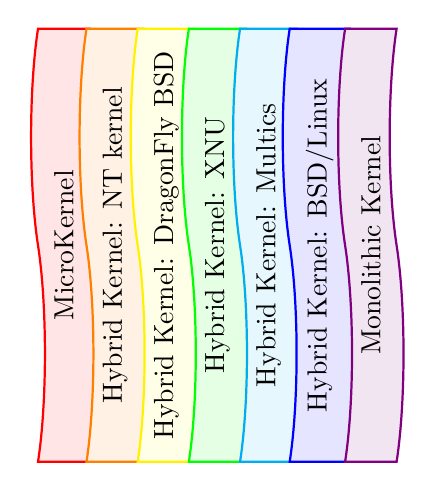
\begin{tikzpicture}[node distance=1mm]

\node [align=center,tape,minimum  width=5.5cm,draw=red,thick,fill=red!10,rotate=90]
{MicroKernel};
\node at (0.65,0) [align=center,tape,minimum  width=5.5cm,draw=orange,thick,fill=orange!10,rotate=90]
{Hybrid Kernel: NT kernel};
\node at (1.3,0)
[align=center,tape,minimum  width=5.5cm,draw=yellow,thick,fill=yellow!10,rotate=90]
{Hybrid Kernel: DragonFly BSD};
\node at (1.95,0)
[align=center,tape,minimum  width=5.5cm,draw=green,thick,fill=green!10,rotate=90]
{Hybrid Kernel: XNU};
\node at (2.6,0)
[align=center,tape,minimum  width=5.5cm,draw=cyan,thick,fill=cyan!10,rotate=90]
{Hybrid Kernel: Multics};
\node at (3.25,0)
[align=center,tape,minimum  width=5.5cm,draw=blue,thick,fill=blue!10,rotate=90]
{Hybrid Kernel: BSD/Linux};
\node at (3.9,0)
[align=center,tape,minimum  width=5.5cm,draw=violet,thick,fill=violet!10,rotate=90]
{Monolithic Kernel};

\end{tikzpicture}

\end{document}
